\section{Memories}
\label{sec_memories}


%MAIN INSIGHTS: 
%1 - Figure~\ref{DDRCS}: DDR3 and DDR4 thermal neutrons cross sections. DDR3 and DDR4 have opposite trends for 0-1 and 1-0 bitflips. We have seen both transient, intermittent, permanent fault and SEFIs
%2 - Figure~\ref{DDR}: single and multiple bit distribution shows that ECC could not be sufficient, there is a good amount of multi bit errors induced by neutrons in both DDR3 and DDR4
%3 - Figure~\ref{ddrsc}(next page): We predict the FIT rate of the whole bunch of DDR3 or DDR4 of the 10 fastest supercomputers in the world, considering their memory utilization and their location, simplifying the thermal acceleration factor. We will comment on rainy vs sunny days
%4 - We will compare our estimation with previoulsy published data on DDR FIT rate in some supercomputers

%\begin{figure}[tb]
%\centering
%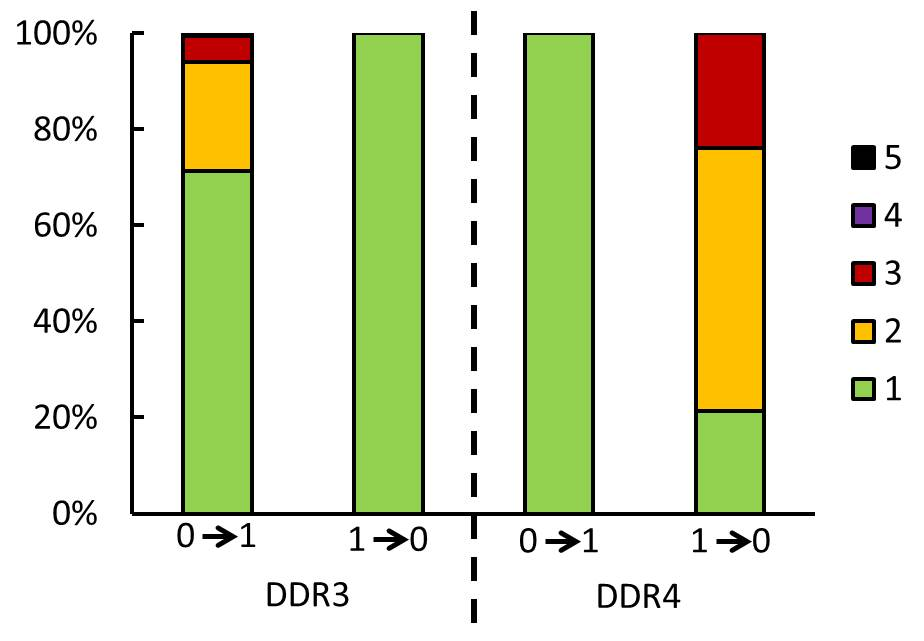
\includegraphics[width=0.9\columnwidth]{./data/plots_final/DDR_errors.jpg}
%\caption{DDR3 and DDR4 Single and Multiple Bit Distribution. }
%\label{DDR}
%\end{figure}


%\begin{figure}[tb]
%\centering
%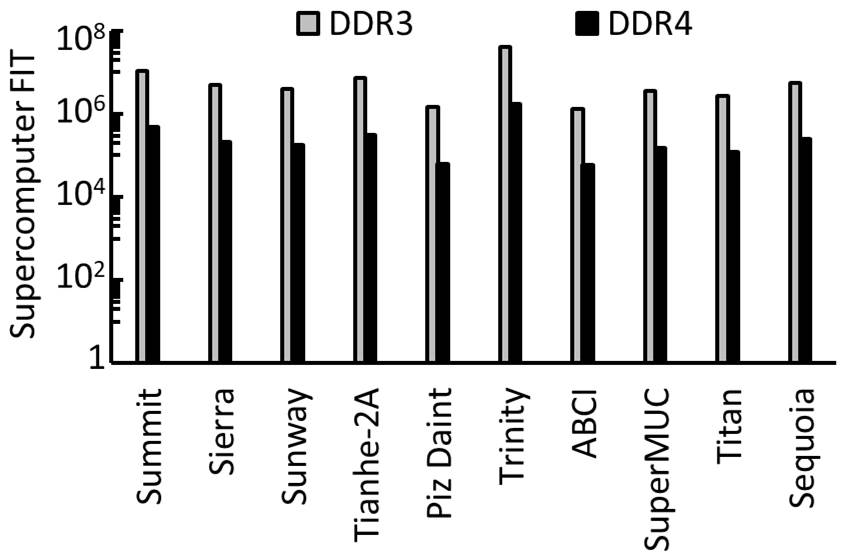
\includegraphics[width=0.9\columnwidth]{./data/plots_final/HPC_FIT.jpg}
%\caption{Predicted DDR3 and DDR4 Thermal FIT rate for the first ten fastest supercomputers from Top500 list.}
%\label{ddrsc}
%\end{figure}

In this section, we present the Double Data Rate (DDR3 and DDR4) Dynamic
Random Access Memories (DRAM) sensitivity to thermal neutrons. Both DDR memories are synchronous DRAM tested without ECC and composed of a single rank x8 memory module. The DDR3 is a 4GB module that operates at 1.5V with a frequency of 1866 MHz and timings 10-11-10. The DDR4 is an 8GB module that operates at 1.2V with a frequency of 2133MHz and timings 13-15-15-28. As vendors are
not explicitly mentioned, cross sections are shown in nominal values. 

We irradiate the devices while performing a continuous read/write \textit{correct loop}: banks are set to 0xFF (or 0x00) and continually read while irradiated with neutrons. When an unexpected value appears, error counters are increased, the corrupted data is downloaded for further analysis, and the memory bank is rewritten. This read/write loop allows differentiating 1-0 and 0-1 bit flips. While Static RAM has a symmetric structure, DDR are likely to be more sensitive to either one of the two possible bit flip directions (one-to-zero and zero-to-one), depending on the cell implementation and on the use of complementary logic.
%The first means the expected value is one and the read value is zero, and the second means the expected value is zero and the read value is one.


The errors are classified into four categories: 
\begin{itemize}[noitemsep]
\item \textbf{Transient error:} a bit flip that does not systematically appear in the following memory read. %That is, incorrect data is read from a memory location but overwritting with correct data. 
%Transient errors in DDR memories have been extensively studied by \cite{baumann2005soft,ziegler1981effect}. 
\item \textbf{Intermittent error:} a memory location returns incorrect values, but not necessarily in consecutive reads. Intermittent errors have been seen in DDR and are dependent on environmental conditions, like temperature~\cite{constantinescu2008intermittent}.
%Abnormal environment conditions, such as elevated temperatures, pollution or cosmic and aplha rays, are responsible for these errors\cite{constantinescu2002impact,sridharan2013feng}. An intermittent error is indicative of device
%damage or malfunction. % In the responsible condition: add cosmic rays and alpha particles.
\item \textbf{Permanent error:} a memory location consistently returns an incorrect value (stuck-at). Permanent errors are caused by Displacement Damage (the neutron dislocates atoms in the transistor) and can possibly be repaired with annealing (i.e., heating the device)~\cite{quinnDDR,srour2003}.
%\cite{constantinescu2003trends}. 

\item \textbf{Single Event Functional Interrupt (SEFI):}  a large portion of the memory array return incorrect values, likely caused by an error in the DDR control logic circuits. Further reads/writes will return correct values~\cite{electronic1996test}.

\end{itemize}

\begin{figure}[tb]
\centering
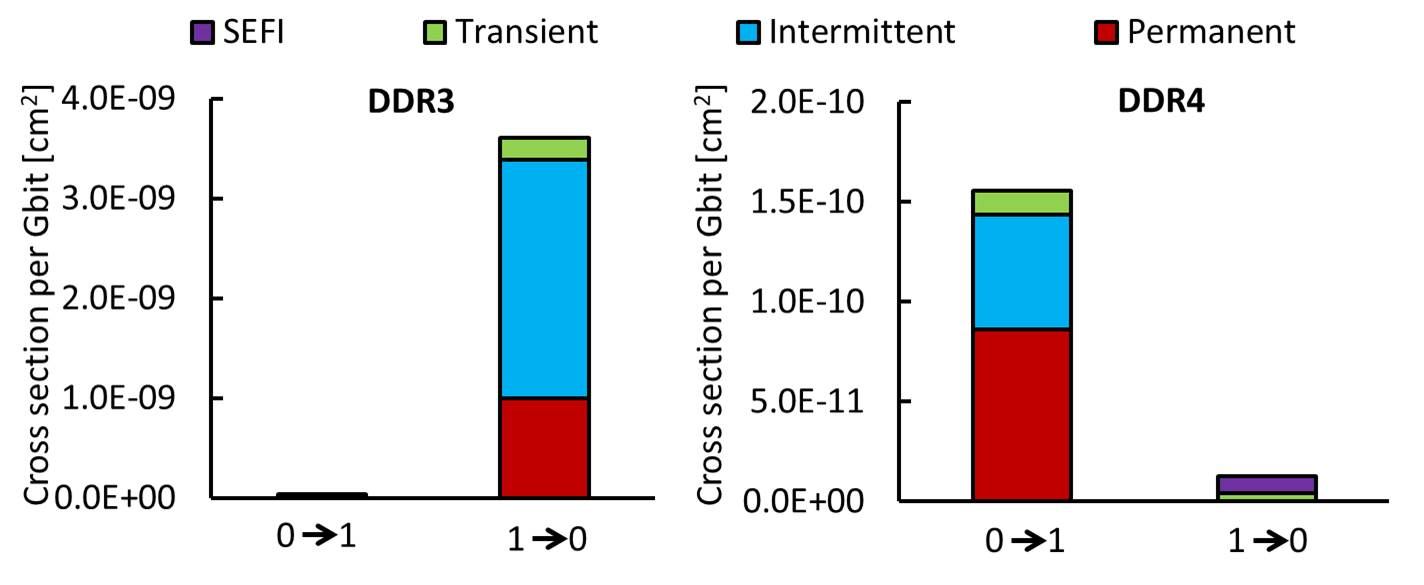
\includegraphics[width=1.00\columnwidth]{./data/plots_final/cs_DDR.jpg}
\caption{DDR3 and DDR4 thermal neutrons cross sections.}
\label{DDRCS}
\end{figure}

Figure~\ref{DDRCS} shows the thermal neutrons cross section per GBit for DDR3 and DDR4. We do not report high energy neutron data since after few minutes of irradiation at ChipIR both DDR3 and DDR4 experienced a high number of permanent faults, impeding further data collection. However, the sensitivity of DDR memories to high energy neutrons has been extensively studied, and experimental data can be found in~\cite{constantinescu2002impact,sridharan2013feng,quinnDDR,guertin2017}.

Figure~\ref{DDRCS} highlights that the DDR4 memory cross section is approximately one order of magnitude lower than the DDR3 one, showing significant reliability improvements probably resulting from new manufacturing processes as well as transistor placement enhancement. We also observe in Figure~\ref{DDRCS} that more than 95\% of all the errors are in one of the two possible bit flip direction, one-to-zero for DDR3 and zero-to-one for DDR4. The opposite direction for DDR3 and DDR4 suggests that one device is manufactured with complementary logic. 
Another interesting point our data highlights is the proportion of each error category changes from DDR3 to DDR4. Permanent errors are more than 50\% of all observed errors in DDR4, while on DDR3 only less than 30\% of errors are permanent. It is also worth noting that both technologies present SEFI errors during the experiments. That is, an impinging particle on both DDR memory control circuits tend to incite similar malfunctioning behaviors.

Finally, all the observed transient and intermittent errors were single bit
flip. This is a promising result, as SECDED ECC is shown to be sufficient to
corrects most thermal neutrons induced errors~\cite{sridharan2012study}. On the contrary, in a SEFI error multiple corrupted bits were observed.


%DDR4 memory errors are less likely to happen but with a greater impact to normal operation;

%Despite presenting better general results, DDR4 memories are more susceptible to radiation-induced permanent errors. That is, DDR4 memories errors generate more critical output corruption as the fault persist on time.
%Intermittent radiation-induced memory errors affect in a greater way the DDR3 device. A possible reason for that is the diminution of voltage operation introduced by DDR4 technology.
% Transient errors appear to remain constant between both tested devices.

%An important result observed is that both technologies present SEFIs errors during the experiments. This is, an impinging particle on both DDR memory control circuits tend to incite similar malfunctioning behaviours.   

 %As SEFI is caused by bit flip in memory control circuits, corrupt data may occur in random and multiple positions.


%Falar sobre erros que não sçao SEFIS então o ECC consegue corregir tudos os erros. Nos sefis não tem o que fazer porque são erros na logica de controle


